This section provides the reader with an overview of Swift Scan. The primary operational aspects of the product, from the perspective of end users, maintainers and administrators, are defined here. The key features and functions found in the product, as well as critical user interactions and user interfaces are described in detail.

\subsection{Features \& Functions}
The product will consist of three major software components including a database system, a mobile application, and a web browser application. In addition, three hardware compononent are needed including an RFID reader, Android phone, and a computer with a web browser. One external element, the Internet, allows the mobile application to connect to our database system.

\vspace{0.5 in}
\begin{figure}[h!]
	\centering
   	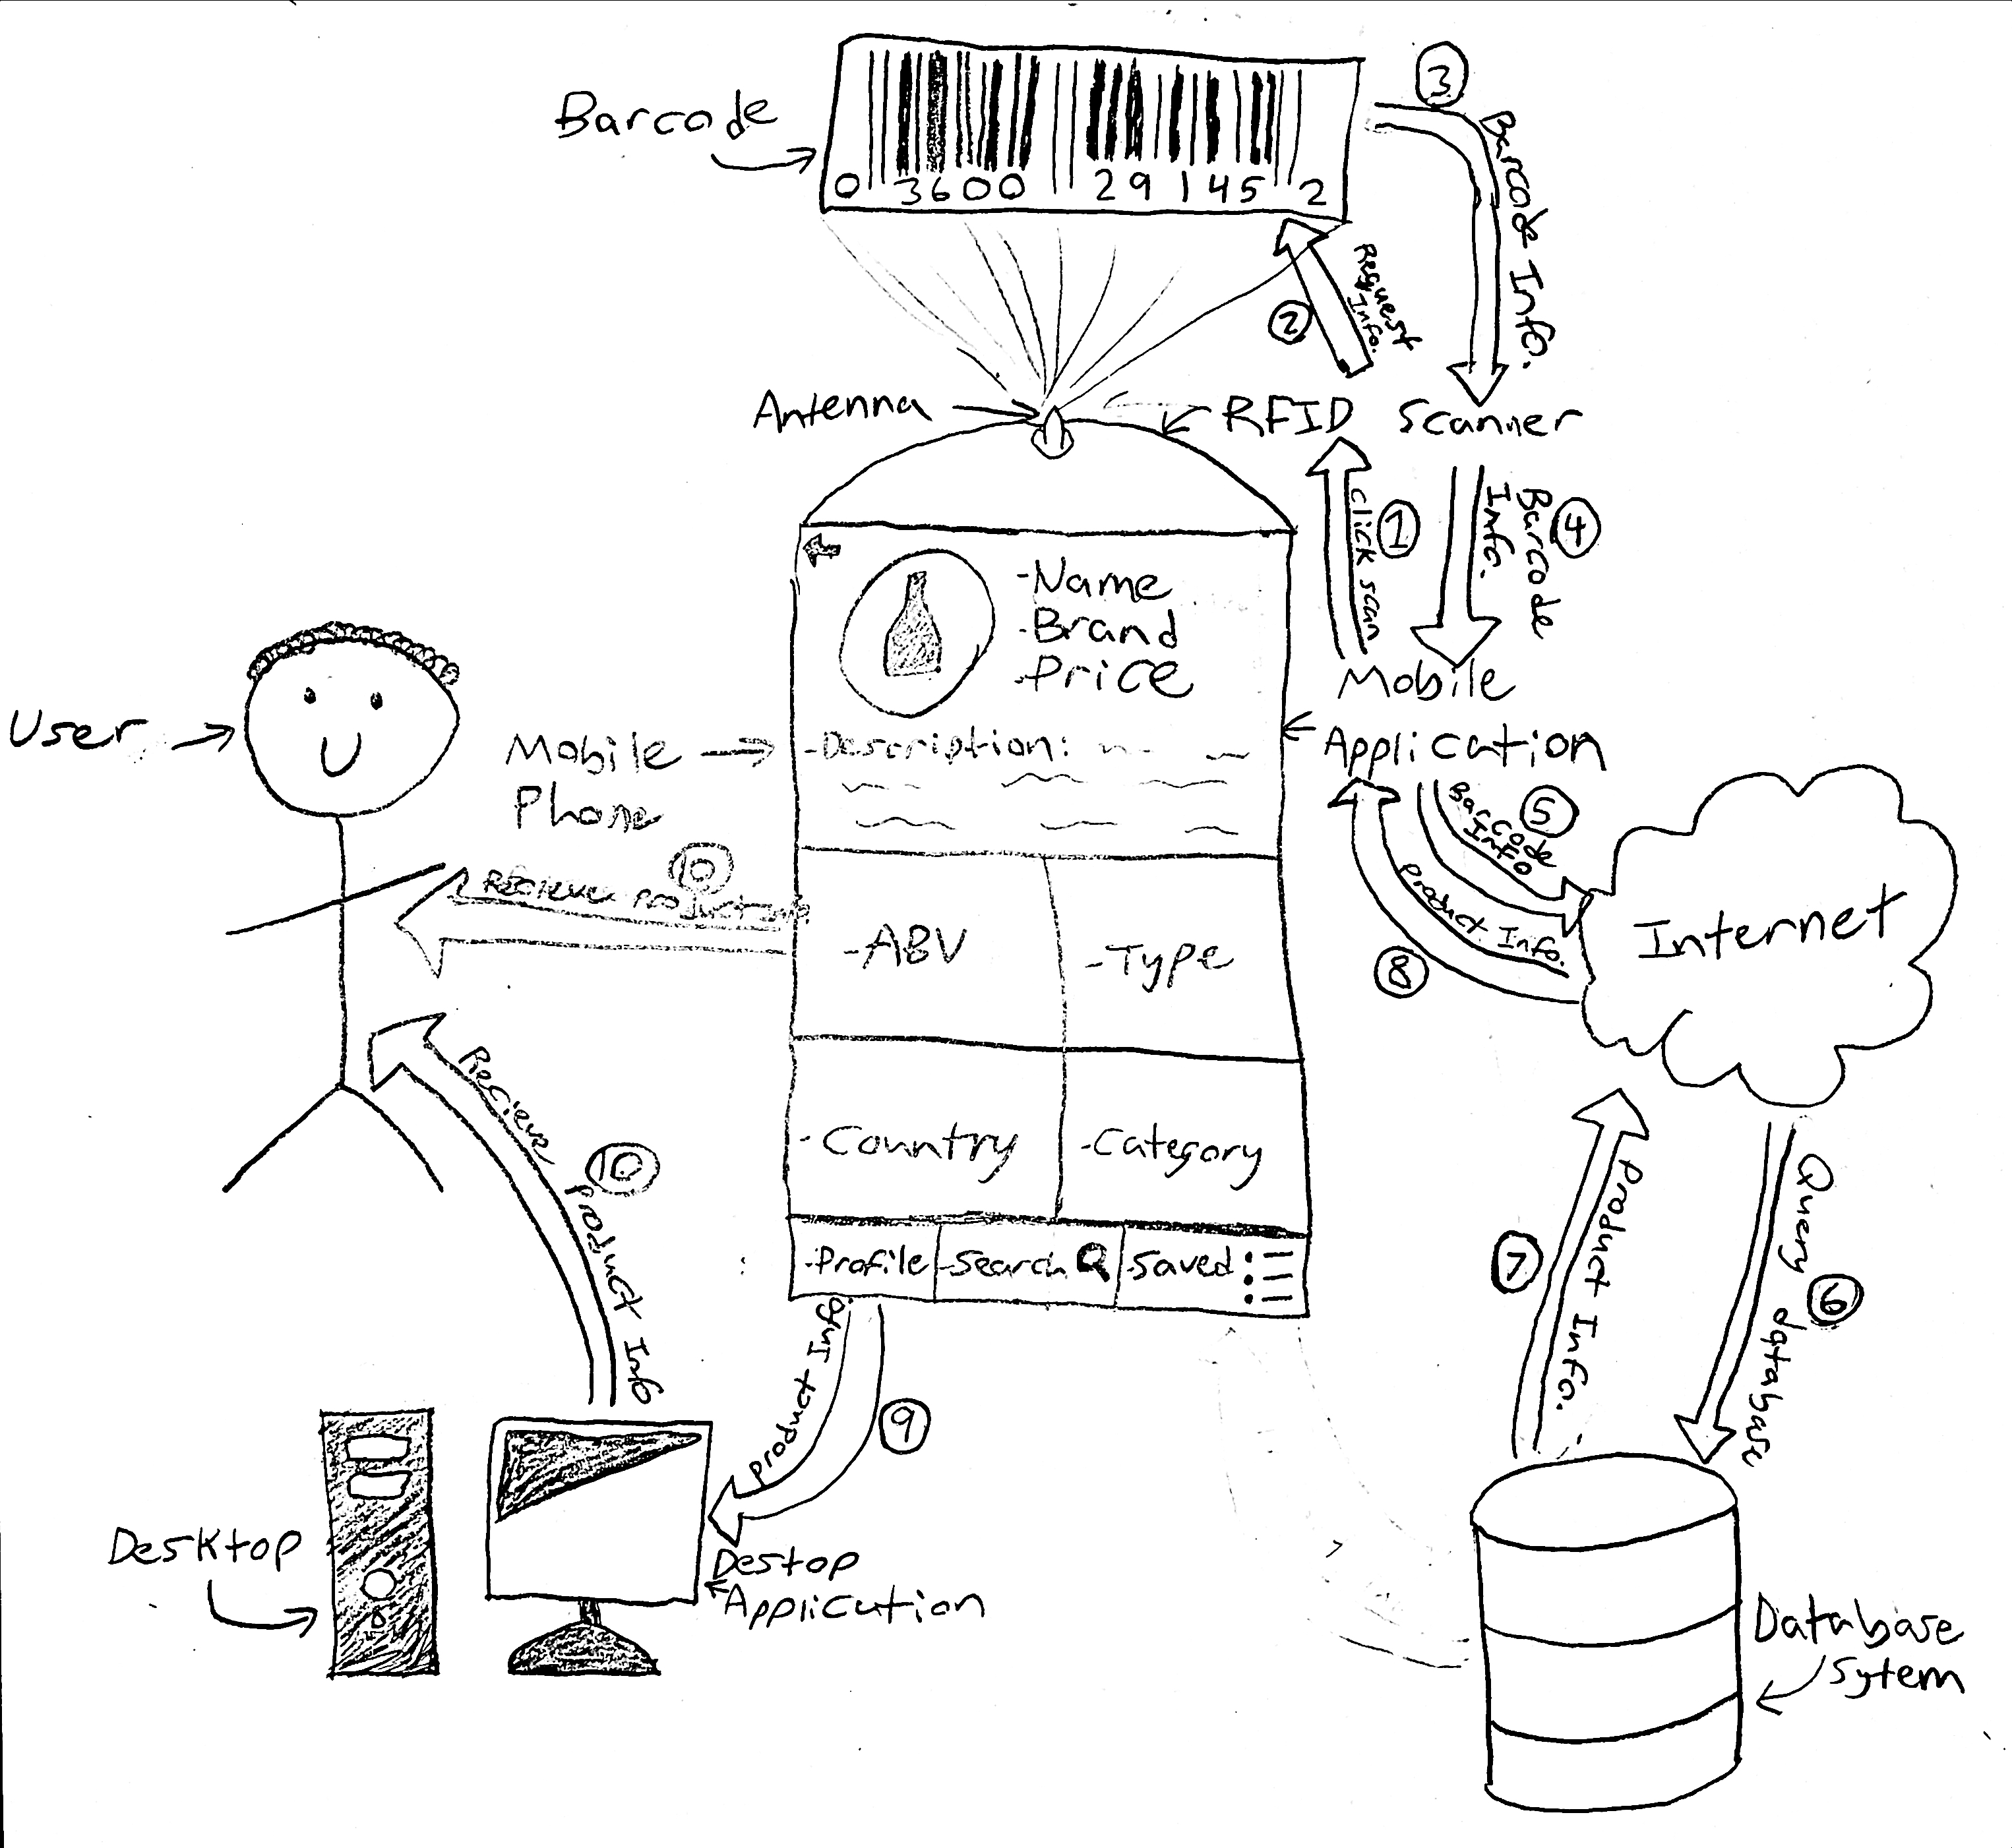
\includegraphics[width=0.60\textwidth]{images/information_flow.jpg}
   	\caption{Information Flow of Swift Scan}
\end{figure}
\vspace{0.5 in}

The main features of the product include:
\begin{itemize}
    \item scans the bar code of any alcoholic beverage
    \item provides information about the product scanned including the brand, alcohol type, category, price (depending on location), ABV, country, etc.
\end{itemize}

\subsection{External Inputs \& Outputs}
Here is a list of data/information flow components:
\begin{itemize}
    \item Barcode Info (Figure 2)
    \begin{itemize}
        \item Description: This information is collected from the barcode by the RFID reader and flows to the mobile phone and then to the database
        \item Use: This will be used to query the database for a product
    \end{itemize}
    \item Product Info (Figure 2)
    \begin{itemize}
        \item Description: This information will be sent from the database system to the mobile to device to be viewed by the user. The information is then synced with the desktop version of the software.
        \item Use: This allows the user to view the information corresponding to the scanned product on their mobile phone or desktop.
    \end{itemize}
\end{itemize}

\subsection{Product Interfaces}
The critical inputs and outputs are the screen to view product information and the camera/RFID reader will allow the user to collect the data. The user will have a simple and easy-to-use interface on their mobile device and desktop browser. The interface will include a profile page, scan page, product page, saved list page, settings, and much more (Figure 3). The administrators will run the database to keep products up-to-date and software like Android studio to make updates. The maintainers will resolve any bugs get reported on GitHub. Here is a mock-up of the mobile interface:
\begin{figure}[h!]
	\centering
   	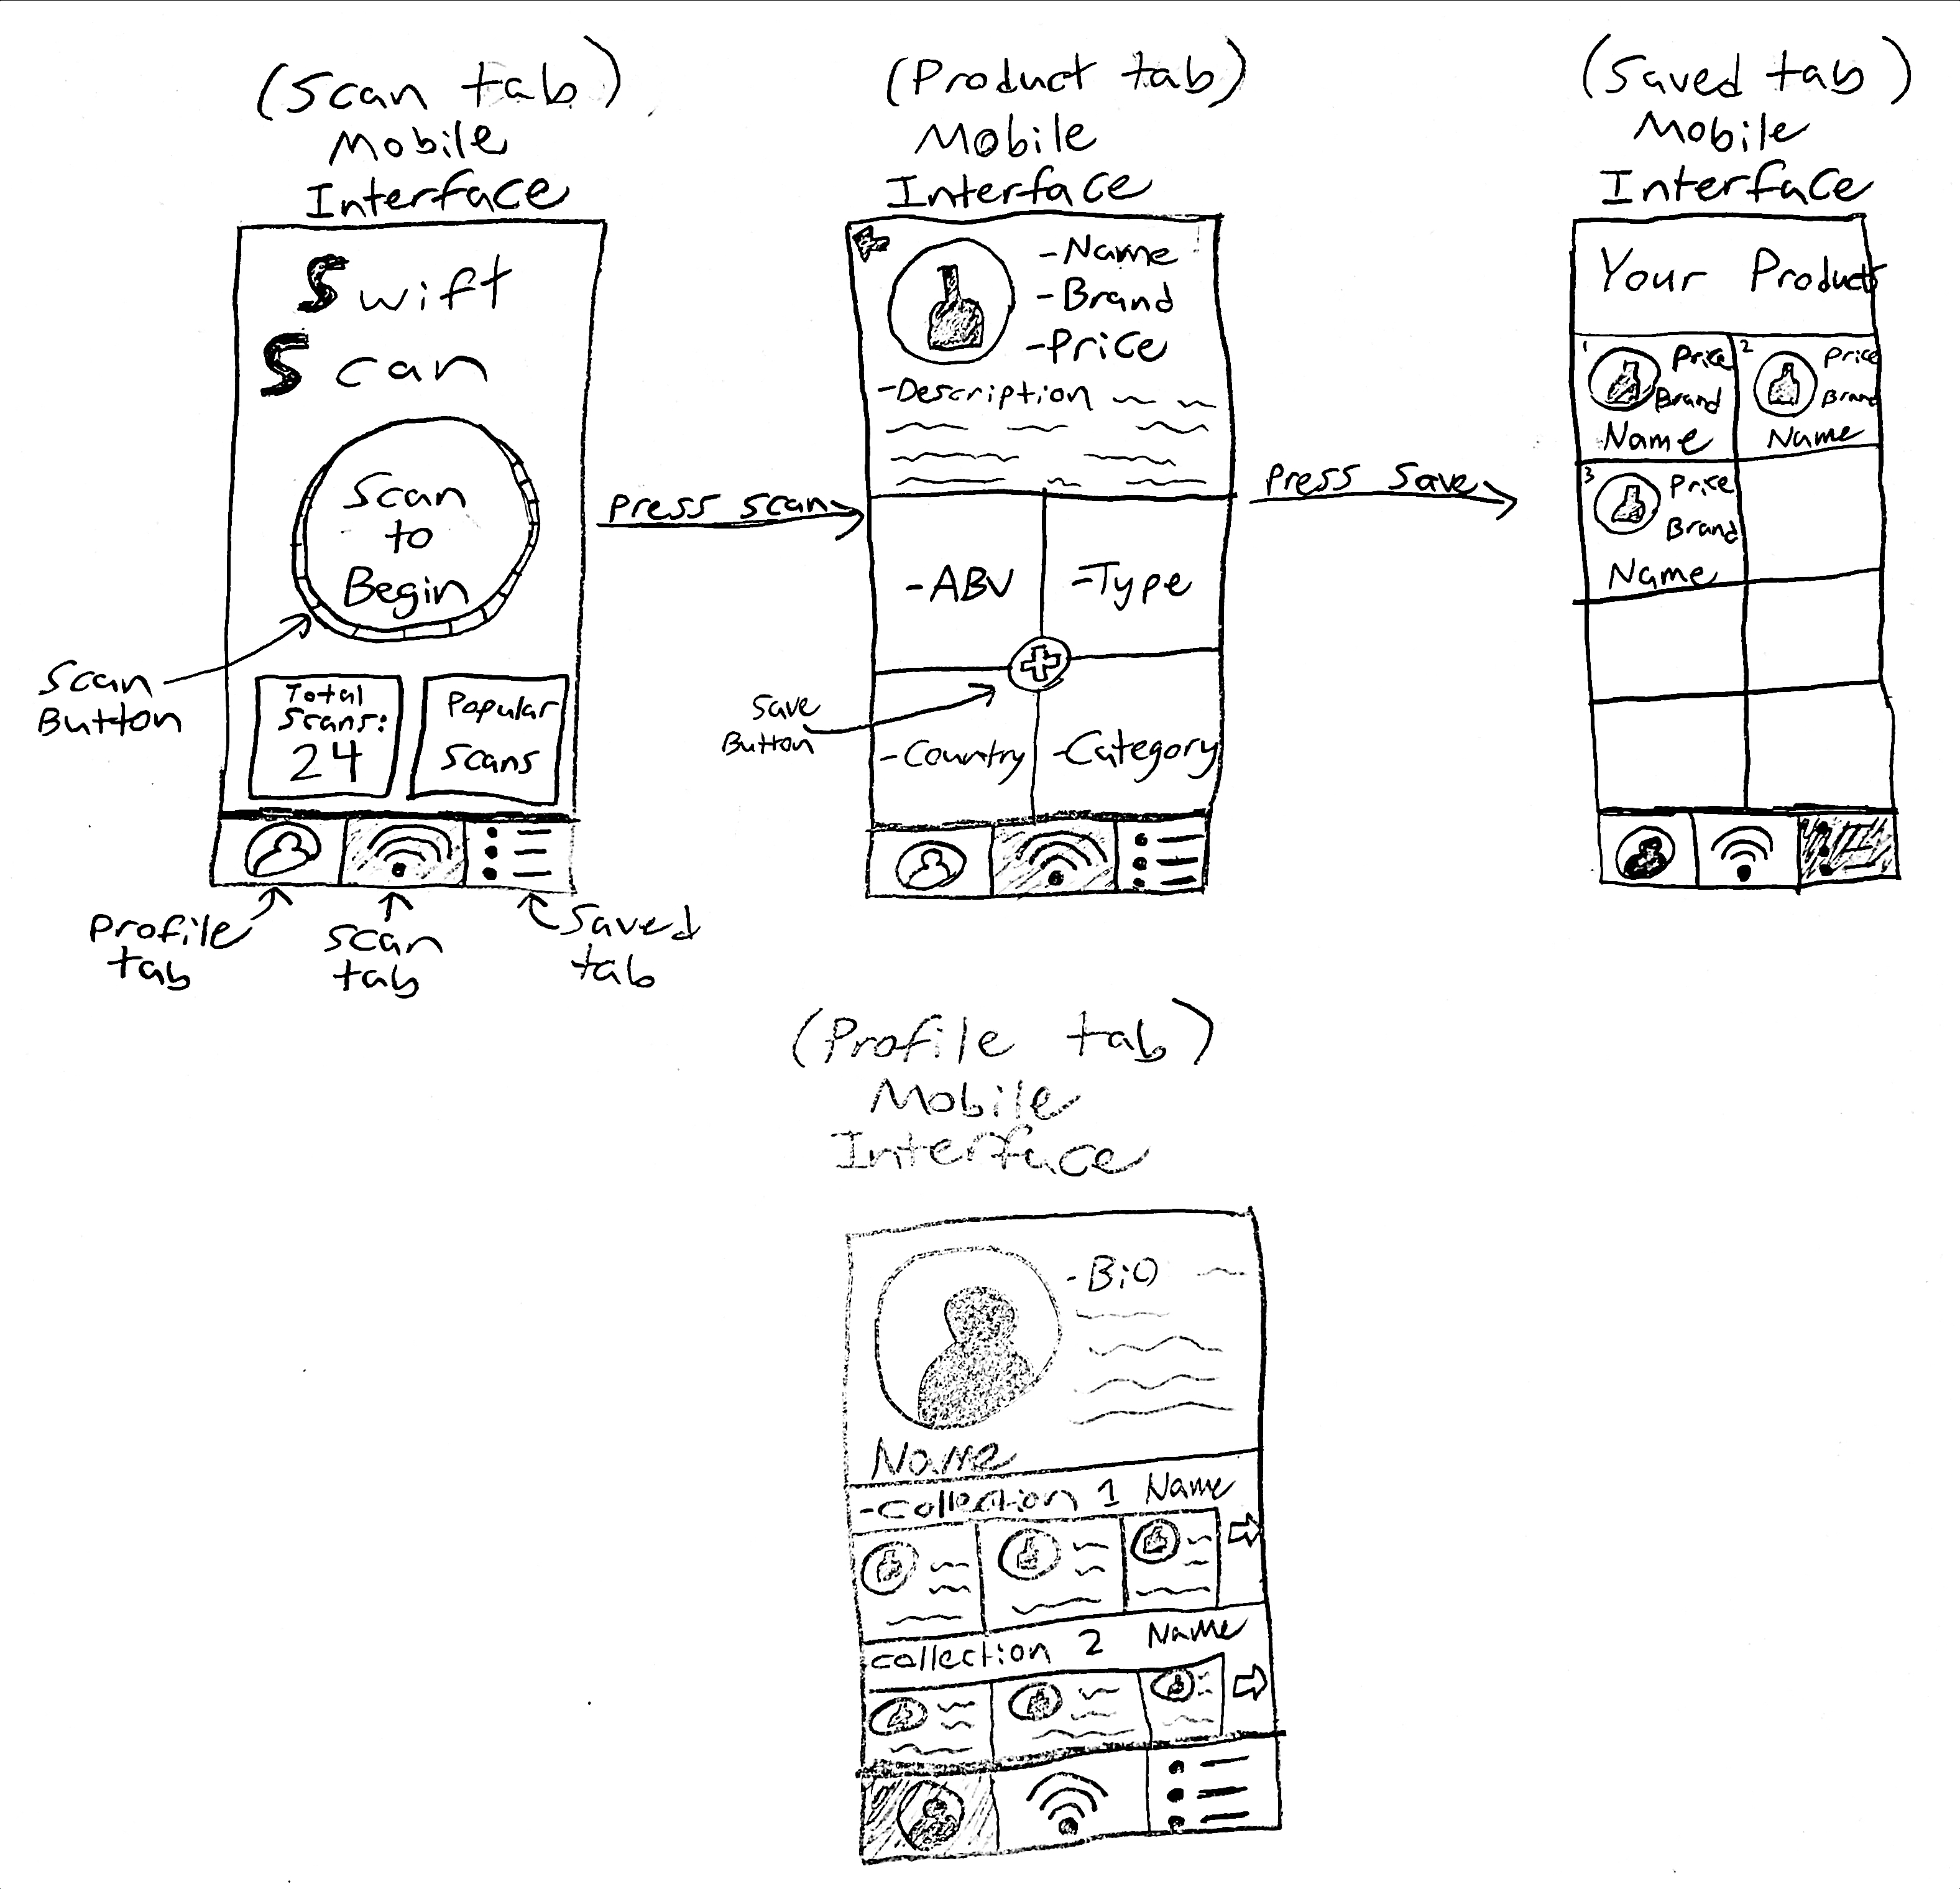
\includegraphics[width=0.60\textwidth]{images/mobile_interface.jpg}
   	\caption{Mobile Interface of Swift Scan}
\end{figure}
